
\documentclass[letterpaper,twocolumn,10pt]{article}
\usepackage{usenix2019_v3}

% to be able to draw some self-contained figs
\usepackage{tikz}
\usepackage{amsmath}

% inlined bib file
\usepackage{filecontents}
\usepackage[noend]{algpseudocode}
\usepackage[ruled]{algorithm2e}

%-------------------------------------------------------------------------------
\begin{filecontents}{\jobname.bib}
%-------------------------------------------------------------------------------
@inproceedings {SLMDB,
author = {Olzhas Kaiyrakhmet and Songyi Lee and Beomseok Nam and Sam H. Noh and Young-ri Choi},
title = {SLM-DB: Single-Level Key-Value Store with Persistent Memory},
booktitle = {17th {USENIX} Conference on File and Storage Technologies ({FAST} 19)},
year = {2019},
isbn = {978-1-939133-09-0},
address = {Boston, MA},
pages = {191--205},
url = {https://www.usenix.org/conference/fast19/presentation/kaiyrakhmet},
publisher = {{USENIX} Association},
month = feb,
}
@article{PCM,
  author    = {H.{-}S. Philip Wong and
               Simone Raoux and
               SangBum Kim and
               Jiale Liang and
               John P. Reifenberg and
               Bipin Rajendran and
               Mehdi Asheghi and
               Kenneth E. Goodson},
  title     = {Phase Change Memory},
  journal   = {Proceedings of the {IEEE}},
  volume    = {98},
  number    = {12},
  pages     = {2201--2227},
  year      = {2010},
  url       = {https://doi.org/10.1109/JPROC.2010.2070050},
  doi       = {10.1109/JPROC.2010.2070050},
  timestamp = {Thu, 08 Jun 2017 09:04:07 +0200},
  biburl    = {https://dblp.org/rec/journals/pieee/WongRKLRRAG10.bib},
  bibsource = {dblp computer science bibliography, https://dblp.org}
}
@misc{3DXPoint,
  author = {Intel},
  title = {Intel and micron produce breakthrough memory technology.},
  note =  {\url{https://newsroom.intel.com/news-releases/intel-and-micronproduce-
breakthrough-memory-technology/}}
}
@misc{NVMRocks,
  author = {NVMRocks},
  title = {RocksDB on Non-Volatile Memory Systems},
  howpublished = {
  \url{http://istc-bigdata.org/index.php/nvmrocks-rocksdb-on-non-volatilememory-systems/}
  }
}
@misc{RocksDB,
  author = {RocksDB},
  title = {RocksDB},
  howpublished = {
  \url{https://rocksdb.org/}
  }
}
@misc{LevelDB,
  author = {Google},
  title = {LevelDB},
  howpublished = {
  \url{https://github.com/google/leveldb}
  }
}
@inproceedings{DBLP:conf/usenix/XiaJXS17,
  author    = {Fei Xia and
               Dejun Jiang and
               Jin Xiong and
               Ninghui Sun},
  editor    = {Dilma Da Silva and
               Bryan Ford},
  title     = {{HiKV}: {A} Hybrid Index Key-Value Store for {DRAM-NVM} Memory Systems},
  booktitle = {2017 {USENIX} Annual Technical Conference, {USENIX} {ATC} 2017, Santa
               Clara, CA, USA, July 12-14, 2017},
  pages     = {349--362},
  publisher = {{USENIX} Association},
  year      = {2017},
  url       = {https://www.usenix.org/conference/atc17/technical-sessions/presentation/xia},
  timestamp = {Mon, 16 Jul 2018 15:47:23 +0200},
  biburl    = {https://dblp.org/rec/conf/usenix/XiaJXS17.bib},
  bibsource = {dblp computer science bibliography, https://dblp.org}
}
@inproceedings{DBLP:conf/fast/LeeLSNN17,
  author    = {Se Kwon Lee and
               K. Hyun Lim and
               Hyunsub Song and
               Beomseok Nam and
               Sam H. Noh},
  editor    = {Geoff Kuenning and
               Carl A. Waldspurger},
  title     = {{WORT:} Write Optimal Radix Tree for Persistent Memory Storage Systems},
  booktitle = {15th {USENIX} Conference on File and Storage Technologies, {FAST}
               2017, Santa Clara, CA, USA, February 27 - March 2, 2017},
  pages     = {257--270},
  publisher = {{USENIX} Association},
  year      = {2017},
  url       = {https://www.usenix.org/conference/fast17/technical-sessions/presentation/lee-se-kwon},
  timestamp = {Tue, 28 Mar 2017 15:26:05 +0200},
  biburl    = {https://dblp.org/rec/conf/fast/LeeLSNN17.bib},
  bibsource = {dblp computer science bibliography, https://dblp.org}
}
@inproceedings{DBLP:conf/usenix/KannanBGAA18,
  author    = {Sudarsun Kannan and
               Nitish Bhat and
               Ada Gavrilovska and
               Andrea C. Arpaci{-}Dusseau and
               Remzi H. Arpaci{-}Dusseau},
  editor    = {Haryadi S. Gunawi and
               Benjamin Reed},
  title     = {Redesigning {LSMs for Nonvolatile Memory} with {NoveLSM}},
  booktitle = {2018 {USENIX} Annual Technical Conference, {USENIX} {ATC} 2018, Boston,
               MA, USA, July 11-13, 2018},
  pages     = {993--1005},
  publisher = {{USENIX} Association},
  year      = {2018},
  url       = {https://www.usenix.org/conference/atc18/presentation/kannan},
  timestamp = {Mon, 16 Jul 2018 15:48:02 +0200},
  biburl    = {https://dblp.org/rec/conf/usenix/KannanBGAA18.bib},
  bibsource = {dblp computer science bibliography, https://dblp.org}
}
@article{LSM-tree,
  author    = {Patrick E. O'Neil and
               Edward Cheng and
               Dieter Gawlick and
               Elizabeth J. O'Neil},
  title     = {The Log-Structured Merge-Tree (LSM-Tree)},
  journal   = {Acta Inf.},
  volume    = {33},
  number    = {4},
  pages     = {351--385},
  year      = {1996},
  url       = {https://doi.org/10.1007/s002360050048},
  doi       = {10.1007/s002360050048},
  timestamp = {Wed, 14 Nov 2018 10:14:19 +0100},
  biburl    = {https://dblp.org/rec/journals/acta/ONeilCGO96.bib},
  bibsource = {dblp computer science bibliography, https://dblp.org}
}
@inproceedings{WiscKey,
  author    = {Lanyue Lu and
               Thanumalayan Sankaranarayana Pillai and
               Andrea C. Arpaci{-}Dusseau and
               Remzi H. Arpaci{-}Dusseau},
  editor    = {Angela Demke Brown and
               Florentina I. Popovici},
  title     = {WiscKey: Separating Keys from Values in SSD-conscious Storage},
  booktitle = {14th {USENIX} Conference on File and Storage Technologies, {FAST}
               2016, Santa Clara, CA, USA, February 22-25, 2016},
  pages     = {133--148},
  publisher = {{USENIX} Association},
  year      = {2016},
  url       = {https://www.usenix.org/conference/fast16/technical-sessions/presentation/lu},
  timestamp = {Tue, 01 Mar 2016 15:34:23 +0100},
  biburl    = {https://dblp.org/rec/conf/fast/LuPAA16.bib},
  bibsource = {dblp computer science bibliography, https://dblp.org}
}
@inproceedings{NVMKV,
  author    = {Leonardo M{\'{a}}rmol and
               Swaminathan Sundararaman and
               Nisha Talagala and
               Raju Rangaswami},
  editor    = {Shan Lu and
               Erik Riedel},
  title     = {{NVMKV:} {A} Scalable, Lightweight, FTL-aware Key-Value Store},
  booktitle = {2015 {USENIX} Annual Technical Conference, {USENIX} {ATC} '15, July
               8-10, Santa Clara, CA, {USA}},
  pages     = {207--219},
  publisher = {{USENIX} Association},
  year      = {2015},
  url       = {https://www.usenix.org/conference/atc15/technical-session/presentation/marmol},
  timestamp = {Fri, 08 Jul 2016 13:19:10 +0200},
  biburl    = {https://dblp.org/rec/conf/usenix/MarmolSTR15.bib},
  bibsource = {dblp computer science bibliography, https://dblp.org}
}
@inproceedings{PebblesDB,
  author    = {Pandian Raju and
               Rohan Kadekodi and
               Vijay Chidambaram and
               Ittai Abraham},
  title     = {PebblesDB: Building Key-Value Stores using Fragmented Log-Structured
               Merge Trees},
  booktitle = {Proceedings of the 26th Symposium on Operating Systems Principles,
               Shanghai, China, October 28-31, 2017},
  pages     = {497--514},
  publisher = {{ACM}},
  year      = {2017},
  url       = {https://doi.org/10.1145/3132747.3132765},
  doi       = {10.1145/3132747.3132765},
  timestamp = {Tue, 06 Nov 2018 16:59:32 +0100},
  biburl    = {https://dblp.org/rec/conf/sosp/RajuKCA17.bib},
  bibsource = {dblp computer science bibliography, https://dblp.org}
}
@inproceedings{Dynamo,
  author    = {Giuseppe DeCandia and
               Deniz Hastorun and
               Madan Jampani and
               Gunavardhan Kakulapati and
               Avinash Lakshman and
               Alex Pilchin and
               Swaminathan Sivasubramanian and
               Peter Vosshall and
               Werner Vogels},
  editor    = {Thomas C. Bressoud and
               M. Frans Kaashoek},
  title     = {Dynamo: amazon's highly available key-value store},
  booktitle = {Proceedings of the 21st {ACM} Symposium on Operating Systems Principles
               2007, {SOSP} 2007, Stevenson, Washington, USA, October 14-17, 2007},
  pages     = {205--220},
  publisher = {{ACM}},
  year      = {2007},
  url       = {https://doi.org/10.1145/1294261.1294281},
  doi       = {10.1145/1294261.1294281},
  timestamp = {Wed, 14 Nov 2018 10:55:11 +0100},
  biburl    = {https://dblp.org/rec/conf/sosp/DeCandiaHJKLPSVV07.bib},
  bibsource = {dblp computer science bibliography, https://dblp.org}
}
@inproceedings{Bigtable,
  author    = {Fay Chang and
               Jeffrey Dean and
               Sanjay Ghemawat and
               Wilson C. Hsieh and
               Deborah A. Wallach and
               Michael Burrows and
               Tushar Chandra and
               Andrew Fikes and
               Robert Gruber},
  editor    = {Brian N. Bershad and
               Jeffrey C. Mogul},
  title     = {Bigtable: {A} Distributed Storage System for Structured Data (Awarded
               Best Paper!)},
  booktitle = {7th Symposium on Operating Systems Design and Implementation {(OSDI}
               '06), November 6-8, Seattle, WA, {USA}},
  pages     = {205--218},
  publisher = {{USENIX} Association},
  year      = {2006},
  url       = {http://www.usenix.org/events/osdi06/tech/chang.html},
  timestamp = {Wed, 04 Jul 2018 13:06:35 +0200},
  biburl    = {https://dblp.org/rec/conf/osdi/ChangDGHWBCFG06.bib},
  bibsource = {dblp computer science bibliography, https://dblp.org}
}
\end{filecontents}

%-------------------------------------------------------------------------------
\begin{document}
%-------------------------------------------------------------------------------

%don't want date printed
\date{}

% make title bold and 14 pt font (Latex default is non-bold, 16 pt)
\title{\Large \bf Improving RocksDB via cache and persistent memory}

%for single author (just remove % characters)
\author{
{\rm Jiannan Cheng}\\
Shanghai Jiaotong University
\and
{\rm Yue Chen}\\
Shanghai Jiaotong University
\and
{\rm Zhicheng Wu}\\
Shanghai Jiaotong University
% copy the following lines to add more authors
% \and
% {\rm Name}\\
%Name Institution
} % end author

\maketitle

%-------------------------------------------------------------------------------
\begin{abstract}
%-------------------------------------------------------------------------------
With the emergence of byte-addressable persistent memory (PM) and commercially available Intel OPTANE NVDIMM, PM offers new opportunities and research directions for improving the performance of key-value (KV) stores. We introduce a feasible solution to improve RocksDB via DRAM-based cache and persistent memory. We replace the DRAM with PM in RocksDB and redesign the memtable, reducing write overhead and providing stronger consistency and faster recovery due to the absence of Write-Ahead-Log (WAL). To optimize the Optimistic Concurrency Control (OCC) in RocksDB, our solution exploits a DRAM-based cache to maintain the sequence number of outstanding transactions, providing validation in memory and avoiding to directly access disk and thus reducing the probability of transaction abort. The cache can also improve read amplification. For Two-Phase Locking (2PL), we simply use the cache to maintain the lock manager. Our expected experimental results show that our solution provides higher read and write performance, faster recovery and lower transaction abort radio compared with RocksDB.
\end{abstract}
%-------------------------------------------------------------------------------


%-------------------------------------------------------------------------------
%-------------------------------------------------------------------------------
\section{Introduction}
%-------------------------------------------------------------------------------

Unlike the relational database, the key-value (KV) database does not need to know the data in the value, so it has higher flexibility. The value can be string, file or picture, and the storage content is diverse. Nowadays, KV stores is widely used in various data intensive applications, such as social network~\cite{RocksDB}, e-commerce~\cite{Dynamo} and network index~\cite{Bigtable}. Log structured merge trees (LSM-tree)~\cite{LSM-tree} is a common way to implement KV stores, such as BigTable~\cite{Bigtable}, LevelDB~\cite{LevelDB} and RocksDB~\cite{RocksDB}. LSM-tree is mainly aimed at write intensive and few query scenarios. The core idea is to give up part of the read performance in exchange for the maximum write performance. Efficient write performance is mainly achieved by constructing a buffer in memory to turn write requests into batch processing, thus turning random writes to disks into sequential writes. In order to ensure the order of data and improve the speed of data access, LSM-tree implements a multi-level data structure, and maintains the data structure through the background thread merge-sort operation (compaction). But it also brings the problem of read and write amplification.

In order to ensure that the system can recover from the failure, Write-Ahead-Log (WAL) is needed to record the operation before writing to memory. After the data is persisted to disk, the log is deleted. Using WAL will cause write performance degradation, so by default, storage systems based on LSM-tree such as LevelDB and RocksDB disable WAL to achieve better performance, but this reduces data consistency, because when crash occurs, some data may be lost.

Because LSM-tree has the problem of read amplification~\cite{WiscKey,NVMKV,PebblesDB}, it is necessary to optimize the concurrency control protocol in KV stores based on LSM-tree. For example, in optimistic concurrency control, in order not to access the data of the disk, the verification phase will only be carried out in memory. If the version data is not in memory, the transaction will abort, which improves the abort rate of the transaction.

With the emergence of byte-addressable persistent memory (PM), there occurs new opportunities and research directions for improving the performance of KV stores. PM has recently become more and more involved in key-value stores \cite{NVMRocks,DBLP:conf/usenix/KannanBGAA18,DBLP:conf/usenix/XiaJXS17}, which ehances the performance of storage system. PM technologies such as PCM~\cite{PCM}, memristors and 3D XPoint~\cite{3DXPoint} promote the rapid development of PM. PM can not only replace disks such as HDDs and SSDs but also be connected via a memory bus and act like DRAM. PM is expected to achieve a comparable read performance with DRAM and the write latency of PM is about 10x higher than DRAM~\cite{DBLP:conf/usenix/XiaJXS17}, but the cost of PM is lower than DRAM. 

In this paper, we use PM to replace the memory components in the RocksDB architecture, and use persistent memory to store memtable and immutable memtable. Because PM has the characteristics of byte-addressability and persistence, it does not need Write-Ahead-Log, reducing the cost of log, and has a stronger consistency. In addition, it has faster recovery speed, because recovery does not need to scan log entry. However, modern CPUs have multiple caches, and in some cases, CPUs may reorder some memory write instructions to improve write performance, which may lead to inconsistent system state. Therefore, we use cacheline flush and memory fence instructions to guarantee the consistency of persistent memory.

In order to optimize the concurrency control of RocksDB, especially Optimistic Concurrency Control (OCC), we use DRAM-based cache to maintain the sequence number of outstanding transactions, so that we only need to validate the sequence number in cache in the validation phase. Since the sequence number is maintained by cache, it has no need to directly access disk and thus no need to abort transaction, which improves read amplification and reduces the rate of transaction abort.

To summarize, we make the following contributions in this paper.
\begin{itemize}
\item We explain the trade-off between performance and consistency in RocksDB and use persistent memory to store memtable and immutable memtable, so it does not require Write-Ahead-Log, which reduces logging costs, has better consistency and faster recovery.
\item We show the limitation of Optimistic Concurrency Control in RocksDB, and use DRAM-based cache to improve read amplification and reduce transaction abort rate.
\item Our expected experimental results show that our solution provides higher read and write performance, faster recovery and lower transaction abort rate compared with RocksDB.
\end{itemize}

The remainder of this paper is organized as follows. Section 2 gives an introduction on persistent memory technologies for KV store and the structure and features of RocksDB with the limitation of WAL overhead and read amplification, explaining the motivation of our work. Section 3 discusses how to leverage persistent memory in RocksDB. Section 4 presents the design details of DRAM-based cache. Section 5 shows the design of experiments and the expected experimental results. At last, Section 6 discusses the related work and Section 7 concludes the paper.
%-------------------------------------------------------------------------------
%-------------------------------------------------------------------------------
\section{Background and Motivation}
In this section, we first discuss the features and background of persistent memory, and the feasibility to replace DRAM with persistent memory. We also present the background and the design of RocksDB~\cite{RocksDB}, providing the limitations of RocksDB.
%-------------------------------------------------------------------------------
\subsection{Persistent Memory}
Persistent Memory, also known as Non-volatile memory(NVM), is a byte-addressable persistent storage device between DRAM and disk in the heterogeneous memory hierarchy. PM can be attached to a memory bus socket just like DRAM, which enables it to be accessed via load and store instructions. Modern PM technologies include phase change memory (PCM)~\cite{PCM}, memristors and 3D XPoint~\cite{3DXPoint}.

Embracing the feature of byte-addressability, PM achieves a comparable read performance with DRAM. However, the write latency of PM is about 10x higher than DRAM~\cite{DBLP:conf/usenix/XiaJXS17}, but the cost of PM is lower than DRAM. These properties make PM a suitable choice for replacing DRAM.

Since the PM can be connected via a memory bus with byte-addressable feature, the PM supports atomic writes of 8 bytes~\cite{DBLP:conf/fast/LeeLSNN17}. Compared with the traditional storage devices using block access, PM supports more fine-grained writes. When writing persistent data, we need to ensure that the data structure is consistent, even in the event of system crash. However, modern CPUs have multiple caches and in some cases, CPUs may reorder some of the memory write instructions to improve write performance, which may lead to inconsistent system state. To keep the PM write order and data structure consistent, we need to explicitly use instructions such as \textbf{MFENCE} and \textbf{CLFLUSH} (Intel x86)~\cite{SLMDB,DBLP:conf/fast/LeeLSNN17,DBLP:conf/usenix/KannanBGAA18} to make memory writes ordered and consistent. In addition, in the case where the size of the data written to the PM is greater than 8 bytes, if the system crashs and performs recovery, the recovered data structure may be partially updated, resulting in inconsistent state. Techniques such as logging and Copy-on-Write (CoW) can be used to handle this situation.


As a new storage device, PM offers new opportunities and research directions for optimizing KV stores. There are previous studies~\cite{NVMRocks,DBLP:conf/usenix/KannanBGAA18,DBLP:conf/usenix/XiaJXS17} that use PM in KV stores to optimize system performance, which requires to redesign the data structure, such as skiplist~\cite{DBLP:conf/usenix/KannanBGAA18, SLMDB}. In this work, in addition to redesigning RocksDB's~\cite{RocksDB} skiplist, we also introduce DRAM-based cache, which works with PM collaboratively to optimize the performance of the system.
\subsection{RocksDB}
\textbf{RocksDB}~\cite{RocksDB} is a persistent Key-Value store based on Log Structured Merge Tree (LSM-tree)~\cite{LSM-tree}. The architecture is shown in Figure \ref{fig:rocksdb}. LSM-tree consists of two parts: memory and Disk. In memory component, in order to improve the write throughput and change the random write to disk into sequential write, RocksDB first constructs a memory table (memtable) buffer in memory to batch write. The memtable is composed of sorted skiplist. When the data of the memtable reaches a threshold, the memtable is set to immutable, and then a new memtable is created to receive the write request. The immutable table will be flushed to disk through background thread. The disk component consists of multi-level sorted string tables (SSTable), from lowest $L_0$ to highest $L_n$. Except $L_0$, each level has one or more sorted SSTable files, where the key ranges of files at the same level do not overlap. The capacity of each level is limited, but the higher level can contain more SSTable files. The capacity of such a level is generally about 10 times larger than that of the previous level. In order to maintain such hierarchical level and data order, when the size of a level exceeds its limitation, the background thread will perform a merge sort operation (compaction) on the level and the next level, and the data of the two levels will be sorted according to the key value. When the two levels have the same key, the value of the lower level will cover the value of the higher level, so as to ensure the uniqueness of each level's data. (except $L_0$, because immutable memtable is not compacted when it is flushed to disk to increase write throughput, SSTables in $L_0$ can have overlapping key ranges.) Generally speaking, LSM-tree optimizes the write operation and sacrifices certain read performance. However, due to the multi-level structure and data order, the read operation still maintains good performance.
\begin{figure}
    \centering
    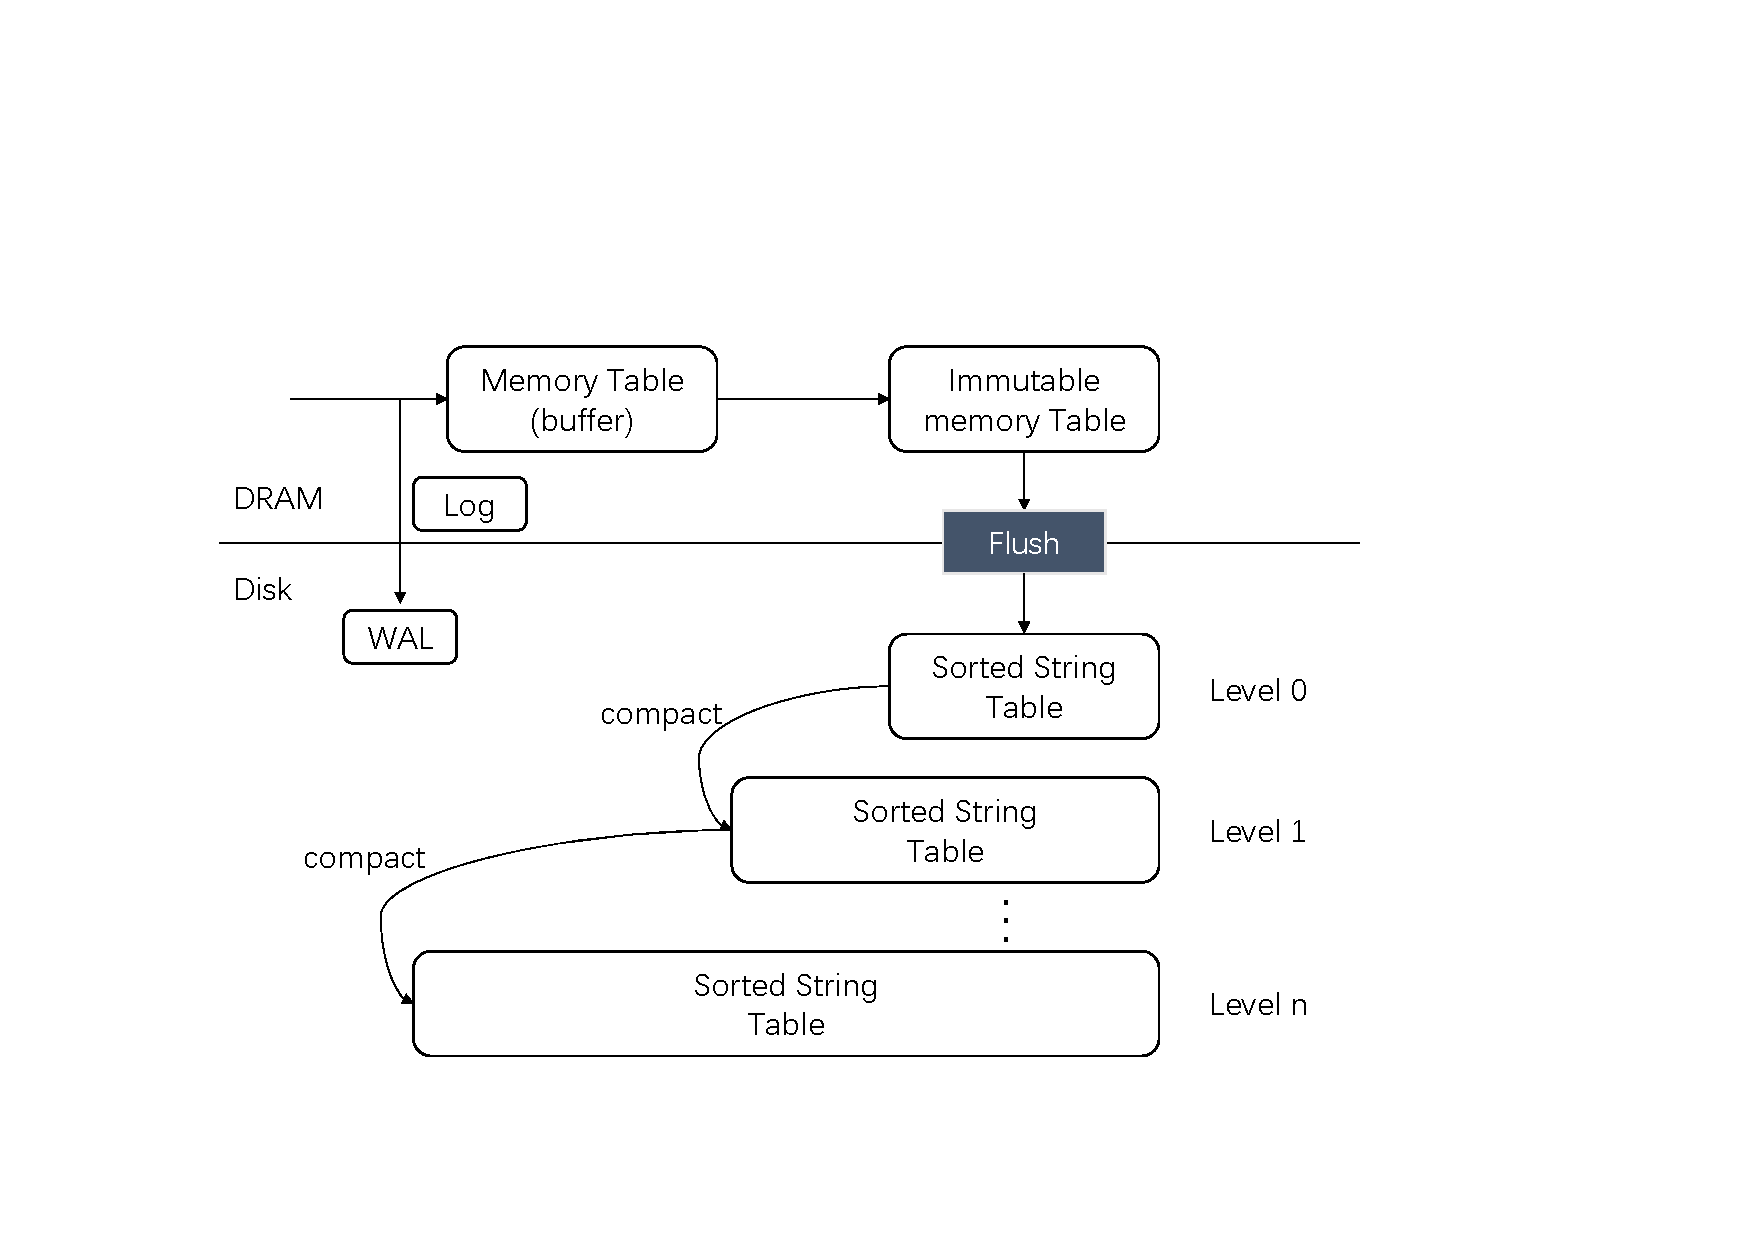
\includegraphics[width=0.36\paperwidth]{figure/rocksdb.pdf}
    \caption{RocksDB architecture.}
    \label{fig:rocksdb}
\end{figure}


\textbf{Write-Ahead-Log overhead} In order to ensure that the system can recover from crash, the write operation will be written to Write-Ahead-Log (WAL) before writing memtable. The log will be deleted after the immutable memtable is finally flushed to the disk. This can cause write performance degradation. When using \texttt{fsync()} for WAL and inserting 8GB of data with 1KB value size to create database, the write performance is reduced by more than 12 times~\cite{SLMDB}. Therefore, the trade-off of performance and consistency is involved here. By default, RocksDB does not log operations to get better performance, so some data may be lost when crash occurs. 

\textbf{Read amplification in transaction} For transactional support, RocksDB supports both Two-Phase Locking (2PL) and Optimistic Concurrency Control (OCC). For 2PL, RocksDB uses a in-memory dedicated locking manager to maintain the locks, decoupling the records with locks. When accessing a record, the manager should be accessed first to acquire lock. 

Because of multi-level structure in LSM-tree, RocksDB has the problem of read amplification~\cite{WiscKey,NVMKV,PebblesDB}. When read operation occurs, it first accesses the memtable, then the immutable memtable. If the data is not in memory, it needs to access the SSTable on disk from the lowest level to the highest level. In each level, it first uses the binary search to find the SSTable where the data is located, after identifying the SSTable, it use another binary search to find the index of the data. Therefore, when retrieving a certain level, at least two binary searches are needed. If the current level cannot retrieve the data, it will go to the next level to search, and repeat the above operations until the data is found, so the overhead of read operation on disk is high. In order to reduce the overhead of accessing the disk, RocksDB uses the Bloom filter to optimize the read operation.

For OCC, verification of records on disk is slow due to the multiple levels on the disk. RocksDB uses the minimum sequence number in memory and global sequence to determine whether to validate in memory. If the sequence is not in memory, the transaction will abort to avoid disk access. In order to optimize the read amplification problem and reduce the probability of transaction abort, we use DRAM-based cache to maintain the sequence number of outstanding transactions, so that we only need to validate the sequence number in cache in the validation phase.


%-------------------------------------------------------------------------------
\section{Design and Implementation of PC-DB}

    \begin{figure}
        \centering
        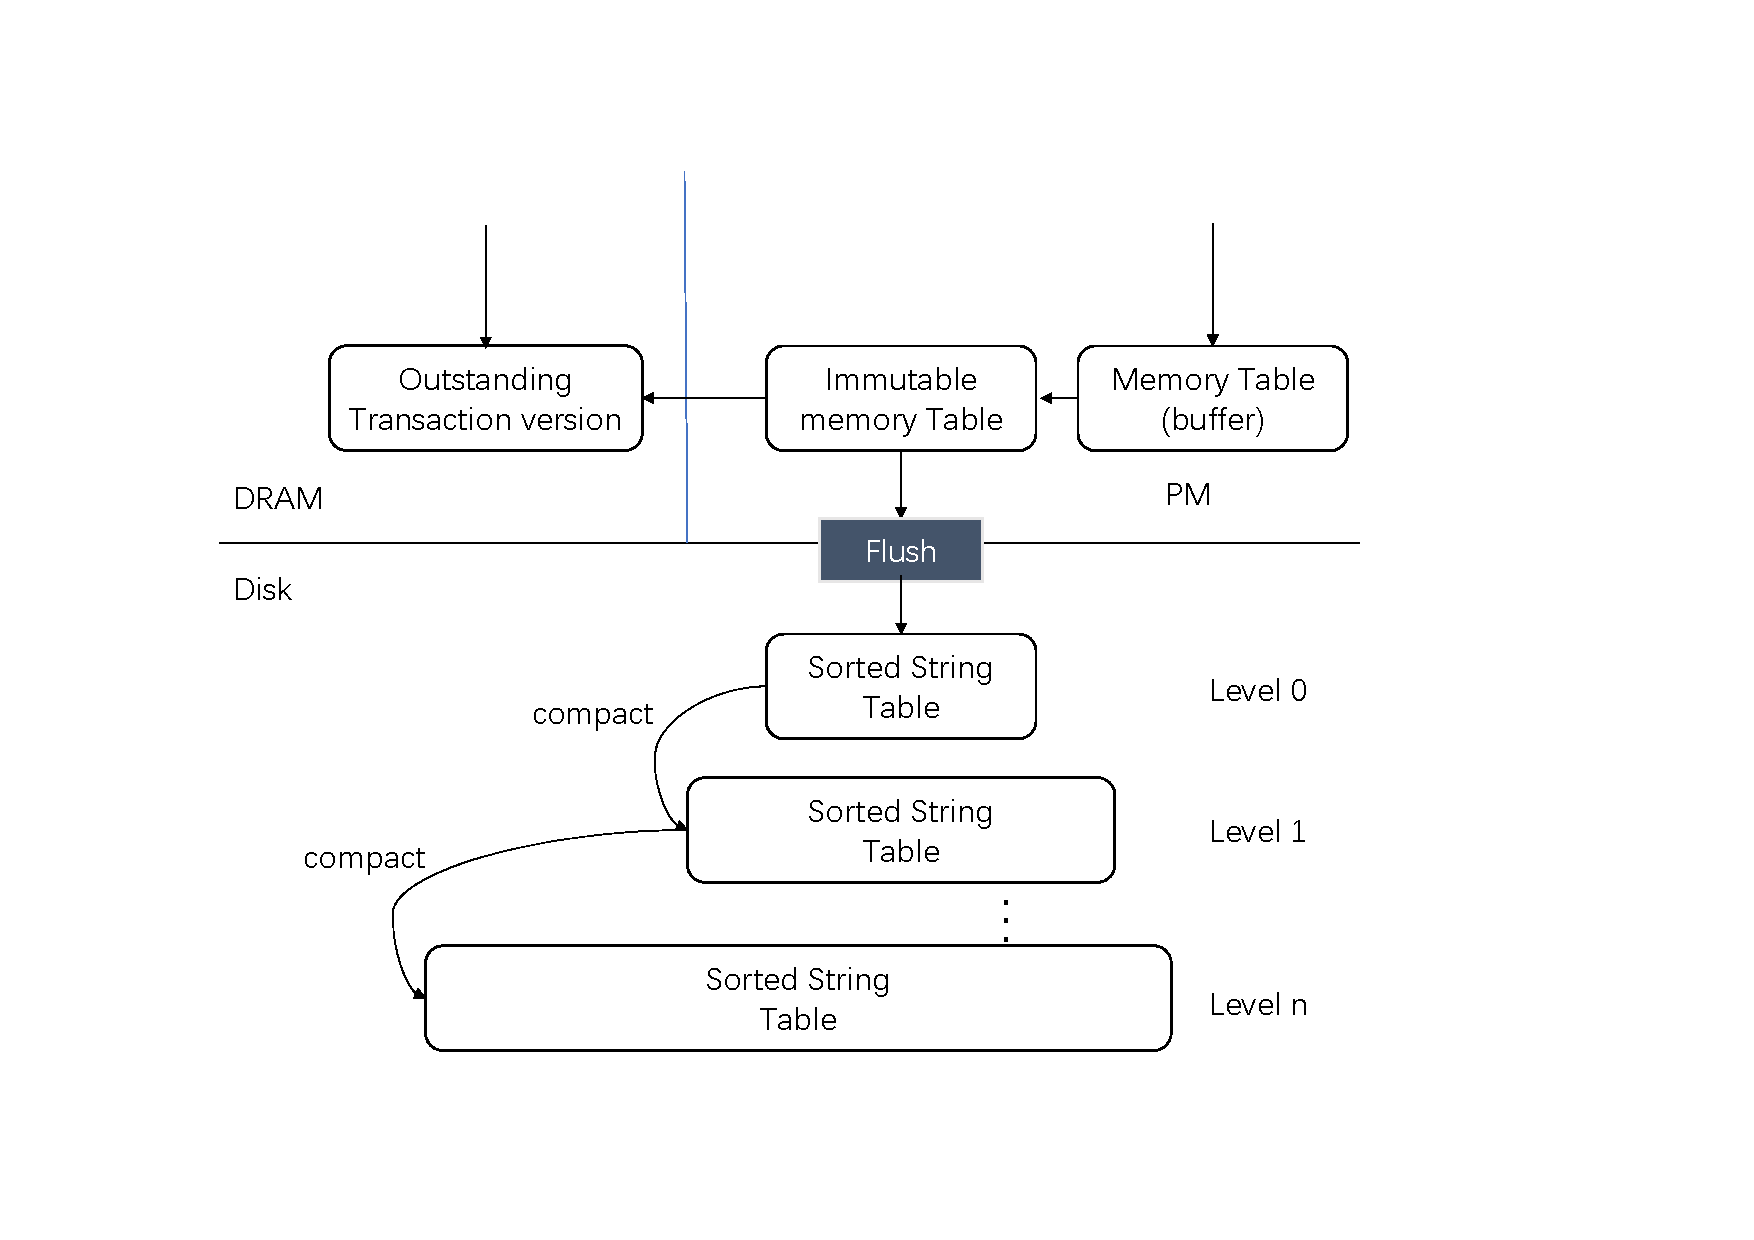
\includegraphics[width=0.36\paperwidth]{figure/structure.pdf}
        \caption{PC-DB architecture.}
        \label{fig:structure}
    \end{figure}
In this section, we present the design and implementation of our work PC-DB, Figure~\ref{fig:structure} shows the overall architecture of PC-DB. PC-DB makes a trade-off between the performance and the consistency, it adopts persistent memory to store MemTable and Immutable Memtable. 
In this way, the Memtable and Immutable Memtable are persistent ,thus eliminating the write ahead log(WAL). 
RocksDB ~\cite{RocksDB} by default disables the WAL in order to provide better performance, 
so persistent Memtable and immutable Memtable in PC-DB will provide stronger durability and consistency upon system failures.

RocksDB adopts OCC for transaction serialization.
For OCC, verification of records on disk is slow due to the multiple levels on the disk. 
RocksDB uses the minimum sequence number in memory and global sequence to determine whether to validate in memory. 
If the sequence is not in memory, the transaction will abort to avoid disk access.
In order to optimize the read amplification problem and reduce the probability of transaction abort, 
we use DRAM-based cache to maintain the sequence number of outstanding transactions, 
so that we only need to validate the sequence number in PM and DRAM in the validation phase instead of serching disk.




\subsection{Persistent MemTable}
MemTable is a skiplist stored in DRAM in RocksDB, which is not persistent. 
It adopts a Write Ahead Log(WAL) for system consistency.
WAL includes the key -value pairs ,version and checksum,which is sequentially appended in the persistent storage. 
However, the overheads of WAL become the bottleneck of write operations and it takes rather long time to recover from crash since it scans long WAL for recovery.

Based on the above problems, we adopt persistent memory for optimization. 
The Memtable is stored in persistent memory ,which avoids the overheads of WAL for consistency and durability. 
The MemTable is a persistent skiplist, which is the same data structure in  RocksDB. As we have talked before, the PM support atomic writes of 8 bytes, 
and in the skiplist, operations like inseration, update, and deletion can all be achieved using a logical inseration operation.
We adopt  $mfence()$ to achieve instruction serialization and $clflush()$ to guarantee that data in cache is flushed into persistent memory and can be recovered under failure. 
Algorithm 1 shows the insert operation. Other operations such as update and delete can also be achieved by logical insert operation.

To put a KV pair into the PC-DB, PC-DB inserts the KV pair along with its version into the MemTable. 
When a memtable is full, it is changed into an immutable. 
Through the compaction of PC-DB, KV pairs will be compressed and written into a new SSTable, the same as RocksDB.


\begin{algorithm}[t]
\caption{Insert(key, value, version,preNode)} %算法的名字


currentNode:=new Node(key,value,version);

mfence();

currentNode.next=preNode.next;

clflush(currentNode);

mfence();

preNode.next:=currentNode;

clflush(preNode.next);

mfence();

\end{algorithm}

Once the system fails, 
the skiplist can be recovered  by locating the root of skiplist, 
the address of which is stored in the MANIFEST file. The PC-DB will also flush the Immutable MemTable if there exits one.
Because the data has already stored in persistent memory,it will be quick compared with recovering from WAL.


\subsection{DRAM-based Cache}
PC-DB uses DRAM as the cache of outstanding transaction version to speed up the version verification in Optimistic Concurrency Control (OCC). This is a space for time strategy.
There are two main methods to mix PM and DRAM memory. The first method is to use DRAM as the cache of PM, and the other method is to use PM and DRAM in parallel,as shown in figure 3. In PC-DB, we choose the second method, which uses DRAM as the cache of outstanding transaction version instead of PM.
\begin{figure}
    \centering
    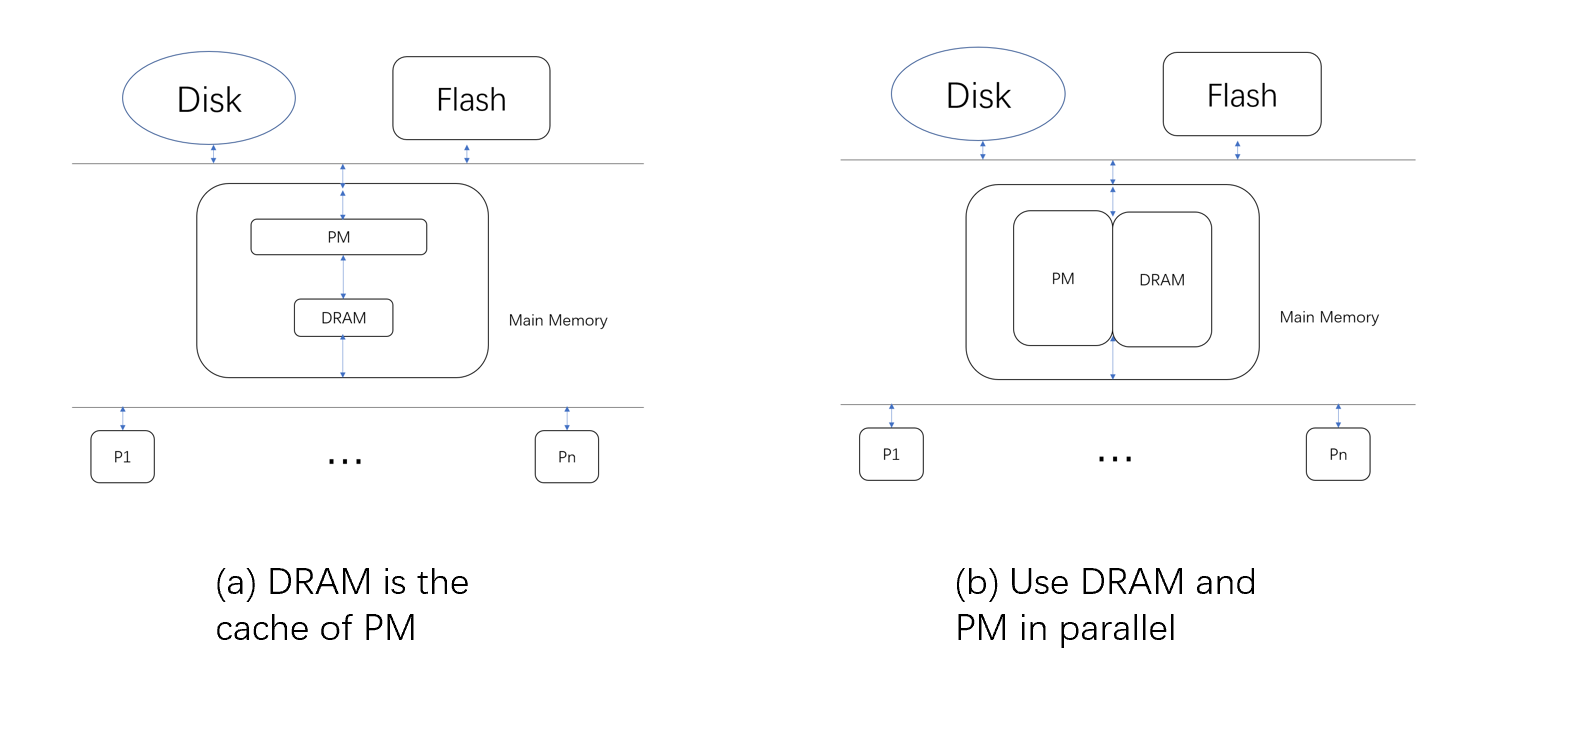
\includegraphics[width=0.36\paperwidth]{USENIX/figure/PM_DRAM.png}
    \caption{Structure of two PM and DRAM mixing methods}
    \label{fig:throughput}
\end{figure}
Take Intel OPTANE DC Persistent Memory\cite{OPTANE} as an example. OPTANE DC Persistent Memory offers two mode: Memory mode and App Direct Mode. When configured to memory mode, application and system sense volatile memory pools. DRAM is used to cache the most frequently accessed data, as well as the PM. It is the first way to mix PM and DRAM. When the App Direct Mode is configured, the application and the operating system clearly know that there are two types of load / storage memory in the platform, and which type of data read / write is suitable for DRAM or Intel OPTANE DC Persistent Memory. Using App Direct Mode, we can store the outstanding transaction version in the DRAM, and use PM to store the MemTable and Immutable MemTable.

Figure 4 shows the algorithm of the Optimistic Concurrency Control of RocksDB. During the commit phase, RocksDB validates the sequence number of each record in the read set. If the latest version of the record does not match the version at the time the record was read, the transaction will abort. There is an observation to introduce the DRAM-based cache: during the commit phase, if the latest version has been flushed into the SSTable, we have to retrieve the record in the SSTable, which will affect the performance due to read amplification. In RocksDB, it maintains the minimal sequence number in the memory, and gets the global sequence number when reading a record. When validating, if the earliest sequence number is smaller than the global sequence number, we only need to validate the version in memory. This approach has some weakness. It will abort some transactions which are legal when the record version has been flushed into the SSTable. There are many approaches to solve this problem. For example, we can attach an index to each record flushed to the disk, but the index will occupy much memory space, which DRAM can't afford. In the OCC optimization, in order to reduce the memory footprint, we do not create an index for each record. What we are concerned with is only the outstanding transaction version, so we can just cache the outstanding transaction version. In PC-DB, DRAM is introduced as the cache. We use the map data structure to store the outstanding transaction version, and we use the App Direct Mode of the Intel OPTANE DC Persistent Memory to store the map in the DRAM. After PC-DB commits a transaction, it should update or add the corresponding records` versions in the DRAM. To validate the version in the read set during the commit phase in OCC, when the version cannot be retrieved in the persistent memory, PC-DB will retrieve  the key in the  DRAM-based cache and obtain the corresponding version if the key exists in the DRAM. However, if the key is not in the DRAM, PC-DB will set the transaction retry after a period of time, and use a background thread to fetch the lasted version of the key from the disk, rather than just abort the transaction. 
\begin{figure}
    \centering
    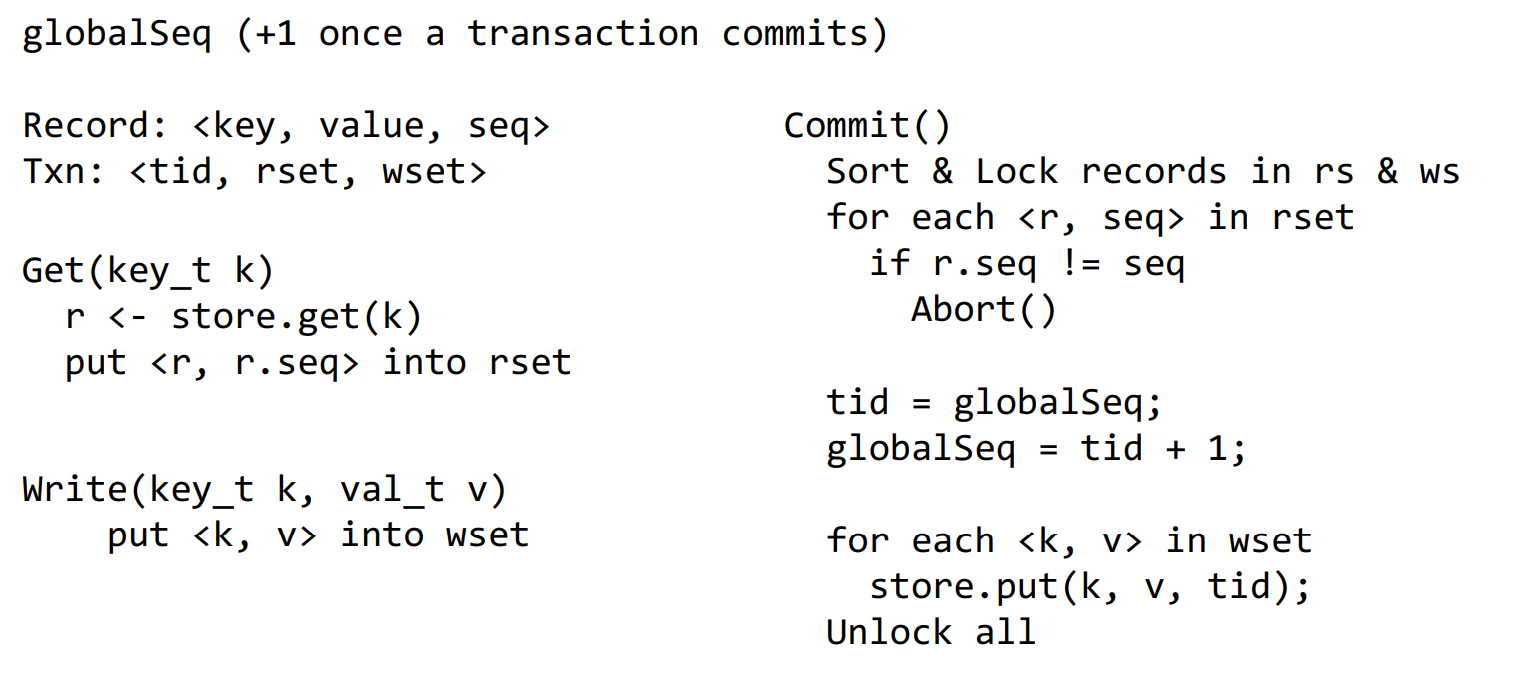
\includegraphics[width=0.36\paperwidth]{USENIX/figure/algorithm.png}
    \caption{Algorithm of the Optimistic Concurrency Control}
    \label{fig:OCCValidation}
\end{figure}
    
\subsection{DRAM Buffer Management}
If PC-DB commits a transaction, it will add the new records' version in the DRAM. Once the DRAM is full, there are several existing strategies to evict the records in the DRAM. One very straight way is to evict the records as soon as the accessing transaction is committed. 
However, if there are other transactions operating on the same records at the same time, they has to wait for the background thread to fetch the versions of the records back to the DRAM, which will take rather a long time. Also, we can  add a reference counter to each of these records in the DRAM. 
If one transaction makes operations on the record, the reference counter will add one, at the same time, if one transaction is committed, 
the reference counter of the records it operates on will minus one. 
When we need to evict some records, we can evict the records whose reference count is zero. 
However, this method will transform the read operation into a write operation, which costs a lot. 
To solve this problem, PC-DB has two approaches. One straight and effective way is to add a timestamp for each of the record in the DRAM. 
When we need to evict some records, we choose these records which are time out. 

Our second approach to evict records in the DRAM uses the LIRS algorithm, 
which performs better than the LRU algorithm. 
The pages in the DRAM are divided into two kinds: the cold pages and the hot pages. 
The division is based on the recent operation frequency. 
When a new record needs to enter into the DRAM but there is no free space, 
PC-DB chooses a cold page and migrate the page that contains the new records to replace the cold page. 
In order to divide the pages in DRAM into cold pages and hot pages, LIRS maintains two sets: Low Inter-reference Recency set and High Inter-reference Recency set. 
Low Inter-reference Recency set contains the pages that are operated on (read and write) frequently within a period of time, while High Inter-reference Recency set contains the cold pages. 
In the LIRS algorithm, two parameters, IRR(inter-reference recency) and Recency, are used . 
IRR is the last two visit intervals of a page, and Recency is how many other pages have been visited since the last visit of the page. 
The IRR and Recency parameters do not contain the number of duplicate pages because the repeated calculation of the page does not have much effect on the priority of current page. 
The division of High Inter-reference Recency set and Low Inter-reference Recency set is based on the IRR, and if two pages have the same IRR, the page with the larger Recency is replaced. 
LIRS algorithm uses stack S and list Q to manage the two set. 
Stack S is used to maintain the hot pages and the potential hot pages, 
and List Q is used to link all the cold pages. 


%-------------------------------------------------------------------------------
\section{Footnotes, Verbatim, and Citations}
%-------------------------------------------------------------------------------

Footnotes should be places after punctuation characters, without any
spaces between said characters and footnotes, like so.%
\footnote{Remember that USENIX format stopped using endnotes and is
  now using regular footnotes.} And some embedded literal code may
look as follows.

\begin{verbatim}
int main(int argc, char *argv[]) 
{
    return 0;
}
\end{verbatim}

Now we're going to cite somebody. Watch for the cite tag. Here it
comes. Arpachi-Dusseau and Arpachi-Dusseau co-authored an excellent OS
book, which is also really funny~\cite{arpachiDusseau18:osbook}, and
Waldspurger got into the SIGOPS hall-of-fame due to his seminal paper
about resource management in the ESX hypervisor~\cite{waldspurger02,SLMDB}.

The tilde character (\~{}) in the tex source means a non-breaking
space. This way, your reference will always be attached to the word
that preceded it, instead of going to the next line.

And the 'cite' package sorts your citations by their numerical order
of the corresponding references at the end of the paper, ridding you
from the need to notice that, e.g, ``Waldspurger'' appears after
``Arpachi-Dusseau'' when sorting references
alphabetically~\cite{waldspurger02,arpachiDusseau18:osbook}. 

It'd be nice and thoughtful of you to include a suitable link in each
and every bibtex entry that you use in your submission, to allow
reviewers (and other readers) to easily get to the cited work, as is
done in all entries found in the References section of this document.

Now we're going take a look at Section~\ref{sec:figs}, but not before
observing that refs to sections and citations and such are colored and
clickable in the PDF because of the packages we've included.

%-------------------------------------------------------------------------------
\section{Floating Figures and Lists}
\label{sec:figs}
%-------------------------------------------------------------------------------


%---------------------------
\begin{figure}
\begin{center}
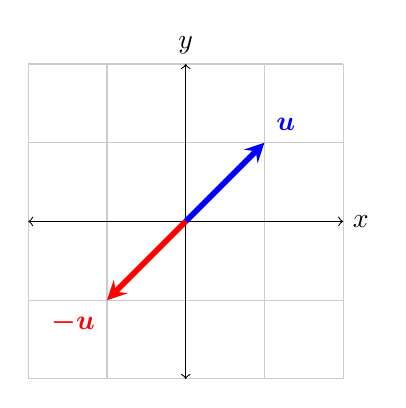
\begin{tikzpicture}
  \draw[thin,gray!40] (-2,-2) grid (2,2);
  \draw[<->] (-2,0)--(2,0) node[right]{$x$};
  \draw[<->] (0,-2)--(0,2) node[above]{$y$};
  \draw[line width=2pt,blue,-stealth](0,0)--(1,1)
        node[anchor=south west]{$\boldsymbol{u}$};
  \draw[line width=2pt,red,-stealth](0,0)--(-1,-1)
        node[anchor=north east]{$\boldsymbol{-u}$};
\end{tikzpicture}
\end{center}
\caption{\label{fig:vectors} Text size inside figure should be as big as
  caption's text. Text size inside figure should be as big as
  caption's text. Text size inside figure should be as big as
  caption's text. Text size inside figure should be as big as
  caption's text. Text size inside figure should be as big as
  caption's text. }
\end{figure}
%% %---------------------------


Here's a typical reference to a floating figure:
Figure~\ref{fig:vectors}. Floats should usually be placed where latex
wants then. Figure\ref{fig:vectors} is centered, and has a caption
that instructs you to make sure that the size of the text within the
figures that you use is as big as (or bigger than) the size of the
text in the caption of the figures. Please do. Really.

In our case, we've explicitly drawn the figure inlined in latex, to
allow this tex file to cleanly compile. But usually, your figures will
reside in some file.pdf, and you'd include them in your document
with, say, \textbackslash{}includegraphics.

Lists are sometimes quite handy. If you want to itemize things, feel
free:

\begin{description}
  
\item[fread] a function that reads from a \texttt{stream} into the
  array \texttt{ptr} at most \texttt{nobj} objects of size
  \texttt{size}, returning returns the number of objects read.

\item[Fred] a person's name, e.g., there once was a dude named Fred
  who separated usenix.sty from this file to allow for easy
  inclusion.
\end{description}

\noindent
The noindent at the start of this paragraph in its tex version makes
it clear that it's a continuation of the preceding paragraph, as
opposed to a new paragraph in its own right.


\subsection{LaTeX-ing Your TeX File}
%-----------------------------------

People often use \texttt{pdflatex} these days for creating pdf-s from
tex files via the shell. And \texttt{bibtex}, of course. Works for us.
%-------------------------------------------------------------------------------
\section{Evaluation}
%-------------------------------------------------------------------------------
\subsection{Methodology}
In evaluation, we use a Dell r740 server with two Intel Xeon E5-2640V3 processors(2.6Ghz), 64GB DRAM, and Intel SSD of 480GB. For PM, we use Intel Optane DC 256 GB Persistent Memory Module, and for the operation system, we use Ubuntu 18.04LTS with Linux kernel version 4.15 is used.
We run PC-DB and RocksDB in this platform by contrast. In PC-DB, we use the APP Direct Mode of Intel Optane DC Persistent Memory Module. In RocksDB and our PC-DB, the MemTable size in RocksDB and PC-DB is set to 64MB, and the key size is set to a fixed size: 20 KB, and all SSTable files are stored in the SSD in both database. 
To evaluate the performance of the two database, we use the db\_bench benchmarks as microbenchmark and the YCSB as real world workload benchmarks.   
\subsection{Using a Persistent MemTable}
Generally our design can be divided into two parts: to get better consistency in exchange of performance, we use PM to replace DRAM; and to improve the read amplification in the validation phase in OCC, we use DRAM to store the outstanding transaction version. In order to better understand what is the effect of the two strategy, we first evaluate the performance of RocksDB,  a modified version of RocksDB by replacing the DRAM using PM, and the PC-DB. Figure 5 shows the expected performance of this evaluation for the random write workload form db$\_$bench over various value sizes. The write latency and total amount of data written to disk is normalized to these of RocksDB.
\begin{figure}
    \centering
    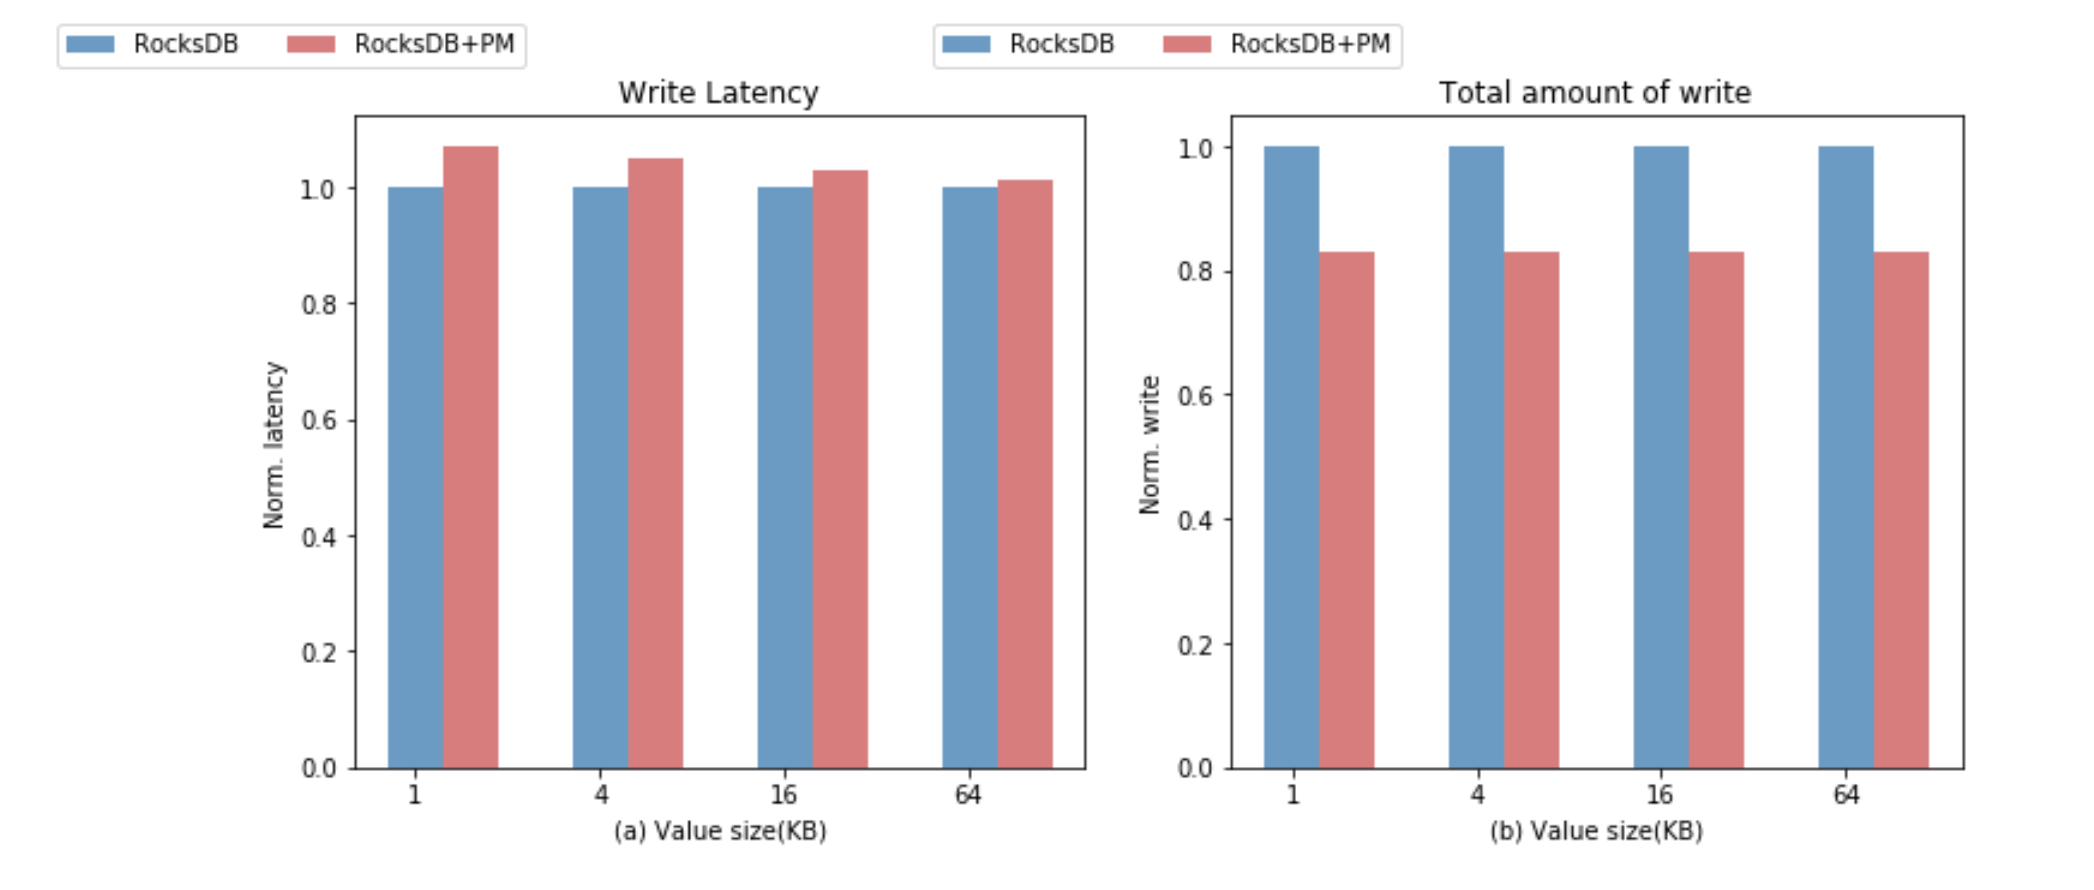
\includegraphics[width=0.36\paperwidth]{figure/Randomwrite.png}
    \caption{Random write performance comparison}
    \label{fig:randomwrite}
\end{figure}
In the figure of write latency, the write latency of RocksDB is similar to that of RocksDB+PM. This is because 1)the write and read latency of PM is higher than the DRAM. 2) RocksDB have to flush WAL to the disk constantly, reducing the performance of RocksDB. However, RocksDB+PM can persistent the inserted data as soon as it is inserted to MemTable, and it can also provide stronger durability. As for the figure of total amount of write, RocksDB+PM can reduce the amount of write data by about $16\%$ compared to the result of RocksDB. This is because RocksDB+PM don`t have to write the WAL. 
\subsection{Result with Microbenchmarks}
Figure 6 shows the operation throughputs of random write and random read workloads of PC-DB, and all of them are normalized to these of RocksDB.
For the random write operations, PC-DB provides almost the same throughput as the RocksDB over all the value sizes. As we have talked before, the write performance of RocksDB is almost the same as RocksDB+PM, and the introducing of DRAM has almost no effect of write performance, because we just need to insert or update the version of the records when a transaction is committed. This overhead of this operation is small. 
For the random operations, PC-DB also shows a similar performance as RocksDB. This because the read latency of PM is almost the same as that of DRAM, and if PC-DB can not get the key in PM, it will search the disk for the recoed, just like the RocksDB.
\begin{figure}
    \centering
    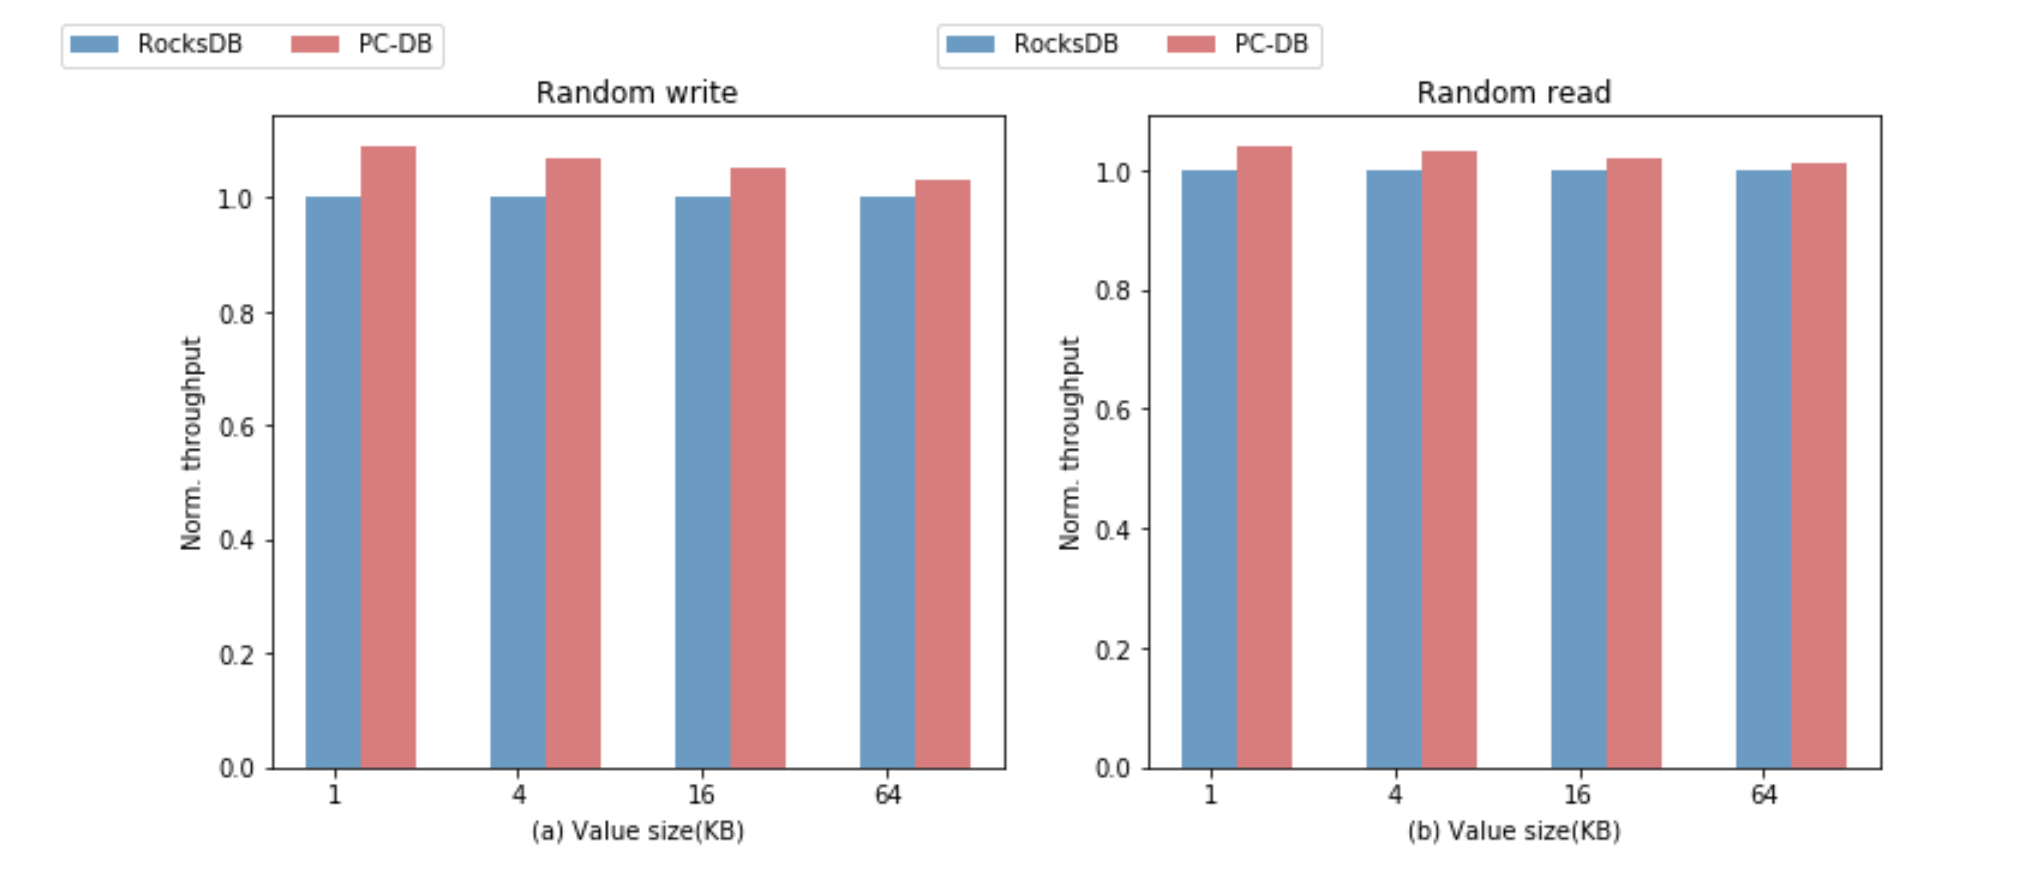
\includegraphics[width=0.36\paperwidth]{figure/Throughput.png}
    \caption{Throughput of PC-DB normalized to RocksDB}
    \label{fig:throughput}
\end{figure}
\subsection{Results with YCSB}
YCSB consists of six workloads. Note that in workload A E, write operation has a more share in the total operations.
\begin{figure}
    \centering
    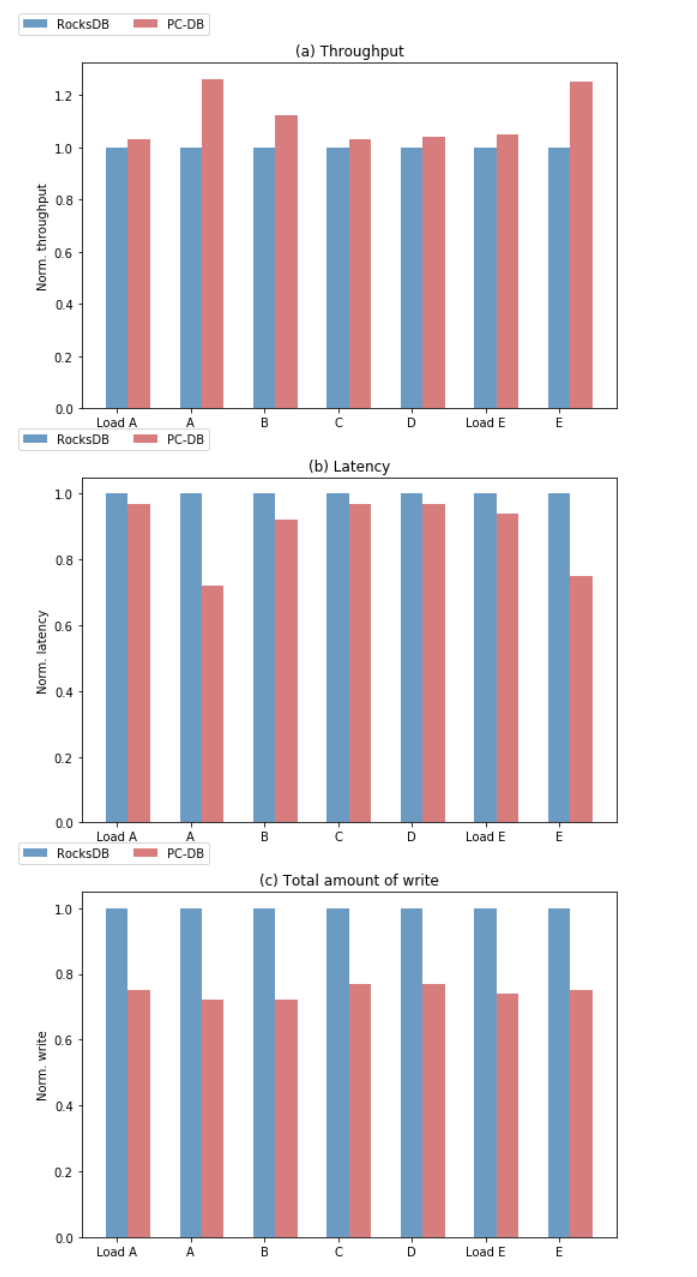
\includegraphics[width=0.36\paperwidth]{figure/YCSB performance.png}
    \caption{YCSB performance }
    \label{fig:YCSB}
\end{figure}
In figure $7(a)$ and $7(b)$, the throughput of PC-DB are higher than those of RocksDB and the latency of PC-DB is smaller than the RocksDB for all workloads, which is because of our using of DRAM as the cache. In the validation phase of OCC, we first search the PM for the latest version of a record, and if it is not found, we search it in the DRAM. While in RocksDB, we have to search the disk for the version if it is not found in the DRAM, which will cost a lot. We can also notice that if the write operations have more shares in the total operations, the PC-DB performs better.
In figure $7(c)$, the total amount of write in PC-DB is much smaller than that of RocksDB for all workloads. this is the same reason as the $5.2$: we don`t have to flush WAL in PC-DB.
%-------------------------------------------------------------------------------
\section{Related Work}
%-------------------------------------------------------------------------------

Previous work, such as skimpystash\cite{skimpystash} and SILT\cite{SILT} ,design KV storage for SSD. 
Skimpystas uses flash as the intermediate cache to store append-only logs, 
so as to benefit from the high sequential write performance of SSD. 
SILT reduces the use of DRAM and maintains a sorted log index in memory by splitting logs across DRAM.
To conclude, these work has increased throughput through batch processing and adding software layers, 
thus enhancing sequencing.

Some previous work has redesigned LSMs for SSD. Wisckey~\cite{WiscKey} redesigned LSMs to reduce read / write amplification and use SSD bandwidth. 
VT-tree\cite{VT-tree} tree design proposes a file system and user level key value storage, which is suitable for workload independent storage. Wang et al.\cite{Wang} exposed I / O channel information of SSDs to leveldb to utilize parallel bandwidth.

NoveLSM\cite{DBLP:conf/usenix/KannanBGAA18} is a persistent KV storage system based on LSM, which aims to utilize non-volatile memory and provide low latency and high throughput for applications. 
It stores the the MemTable and Immutable MemTable in both DRAM and PM for performance and better recovery. 

%-------------------------------------------------------------------------------
\section{Conclusion}
%-------------------------------------------------------------------------------
In this paper, we presented the Persistent-Consistent DB(PC-DB) that use PM to store the MemTable and Immutable MemTable, thus providing faster recovery and better consistency. At the same time, PC-DB make use of the DRAM as a cache for outstanding transaction version, solving the problem of the read amplification in the validation phase of OCC. Our experiments shows that PC-DB performs well in the  YCSB, which are real world workload benchmarks.
%-------------------------------------------------------------------------------
\section*{Acknowledgments}
%-------------------------------------------------------------------------------

The USENIX latex style is old and very tired, which is why
there's no \textbackslash{}acks command for you to use when
acknowledging. Sorry.

%-------------------------------------------------------------------------------
\section*{Availability}
%-------------------------------------------------------------------------------

USENIX program committees give extra points to submissions that are
backed by artifacts that are publicly available. If you made your code
or data available, it's worth mentioning this fact in a dedicated
section.

%-------------------------------------------------------------------------------
\bibliographystyle{plain}
\bibliography{\jobname}

%%%%%%%%%%%%%%%%%%%%%%%%%%%%%%%%%%%%%%%%%%%%%%%%%%%%%%%%%%%%%%%%%%%%%%%%%%%%%%%%
\end{document}
%%%%%%%%%%%%%%%%%%%%%%%%%%%%%%%%%%%%%%%%%%%%%%%%%%%%%%%%%%%%%%%%%%%%%%%%%%%%%%%%

%%  LocalWords:  endnotes includegraphics fread ptr nobj noindent
%%  LocalWords:  pdflatex acks
